\chapter{绪论}
\section{研究背景及意义}

遥感影像变化检测(Remote Sensing Change Detection, RSCD)是遥感领域的核心研究任务之一,主要通过对双时相影像进行比较,识别地表变化~\cite{DQXX202004022}。这一任务对环境监测、灾害评估、资源管理、城市规划与国土安全等多个领域具有至关重要的战略意义。随着遥感技术的飞速发展,我们能够获取的遥感影像在空间分辨率、光谱分辨率和时间分辨率上都得到了前所未有的提升,数据量呈爆炸式增长。因此,如何从海量、高维、多时相的遥感数据中高效、自动化地提取影像中的变化信息并进行精确检测,已成为遥感影像处理领域中的重大挑战~\cite{CHXB201710028}。此外,由于成像时间、季节、光照条件以及传感器参数的差异,双时相影像间常存在大量与真实地物变化无关的“伪变化”,如何有效抑制这些伪变化干扰,增强模型对真实变化的敏感性,是推动变化检测技术走向实用化的关键瓶颈。

\section{国内外研究现状与挑战}
为了应对上述挑战,变化检测算法经历了从传统方法到深度学习方法的持续演进。本章将系统回顾其发展历程,并剖析当前研究所面临的核心挑战。

为了应对上述挑战,变化检测算法经历了从传统方法、结合经典网络模型方法到结合AI大模型的的持续演进。本章将系统地梳理这一发展脉络,并剖析当前研究所面临的核心挑战。本章将从多个关键维度展开回顾:

首先,本章简要分析了传统变化检测方法的基本原理及其局限性,指出其在处理高分辨率遥感影像时面临的挑战。其次,在变化检测的整体架构范式层面,本章将回顾从经典的孪生网络到更复杂的编解码结构的设计演变。通过对这些发展脉络的系统性梳理,本章旨在全面揭示当前变化检测领域的技术前沿、核心挑战与存在的局限。然后,在核心的特征提取架构层面,本章将追溯其从经典的卷积神经网络(CNN),到引入自注意力机制以捕捉长程依赖的Transformer架构,再到近期兼具线性复杂度与全局建模能力的状态空间模型(如Mamba)的演进路径。进一步地,本章探讨多模态表征学习与AI基础模型如何为变化检测任务注入更丰富的语义先验和泛化能力。此外,在变化检测任务中变化表征的关键问题上,本章将剖析几条主流的技术路线,包括数学度量差异表征、交叉自注意力特征交互、模型结构差异表征以及特征交换差异表征。最后,面向变化检测中双时相影像风格差异带来的伪变化问题,本章将综述现有的风格噪声消除的方法,涵盖基于图像预处理、特征对齐、注意力机制以及内容-风格解缠等多种策略。

\subsection{传统变化检测方法}
早期的传统变化检测算法主要依赖于像素级或特征级的数学运算,最具代表性的方法包括影像差值法、比值法和变化向量分析(CVA)等~\cite{YGXB201203010}。这些方法通过直接对比双时相影像的像素值或光谱特征来生成差异图,再通过阈值分割来提取变化区域。此外,还有分类后比较等方法,即先对双时相影像分别进行土地利用分类,再通过比较分类结果来识别变化。然而,这些传统方法严重依赖于手工设计的特征和固定的阈值,对光照和大气噪声极为敏感,且难以处理复杂地物和非线性变化,在面对高分辨率遥感影像时,其精度和鲁棒性往往难以满足应用需求~\cite{Peng2025DeepLC,Ding2025ASO}。

\subsection{遥感影像变化检测任务特征提取架构发展历程}

\subsubsection{基于卷积神经网络的变化检测特征提取研究现状}
深度卷积神经网络在遥感影像变化检测中已经取得了显著成功。CNN能够自动学习图像的层次化特征,有效捕获像素间复杂的空间模式和局部相关性,相比传统手工特征方法性能更佳。由于变化检测任务特有的双时相影像输入,因此典型的CNN式变化检测网络往往采用双分支架构(Siamese CNN):对比前后时相影像的特征来判断变化。其中常用设计包括孪生编码-差异特征计算-解码结构,通常在特征融合阶段还会使用特征金字塔融合策略,以获取不同尺度下的变化信息。近年来,许多研究人员从 CNN 的特征提取强化的角度出发来构建变化检测模型。

针对于变化检测模型中的特征强化,Huang 等人提出结合 EfficientNet-B4~\cite{tan_efficientnet_2019} 构建的变化检测模型~\cite{Huang_RemoteSens_2023_v15_p3972}。该模型通过使用 EfficientNet-B4 作为特征提取器,能够有效地捕捉遥感影像中的细节特征,并通过多尺度特征融合来增强变化检测的精度。Wei 等人提出结合 ConvNeXt~\cite{Liu2022ACF} 模型的变化检测模型~\cite{wei_robust_2024}。ConvNeXt 是一种纯卷积神经网络架构,通过借鉴 Transformer 中的大卷积核、分层规范化(LayerNorm)和渐进式下采样等设计,在保持计算效率的同时大幅提升了特征表达能力。Zhang 等人提出结合 HRNet~\cite{Wang2019DeepHR} 模型的变化检测模型ADHR-CDNet~\cite{Zhang2022ADHRCDNetAD}。在ADHR-CDNet中,基于 HRNet 架构的新型高分辨率骨干网络,用于提取多级和多尺度的实质性变化特征。具有四个不同分辨率相互连接的子网络分支的骨干结构有助于提取多级和多尺度特征。

尽管基于 CNN 架构的变化检测模型得到了广泛的发展和应用,但是由于卷积计算的感受野有限,纯CNN模型难以自适应地建模影像中的全局上下文关系。当变化区域与环境背景存在长距离依赖或同类目标在不同位置发生变化时,CNN可能无法有效区分“真正的变化”与“伪变化”。这导致有时会错误地将季节性差异、光照变化当作变化信号。此外,要覆盖大范围区域,CNN通常需要加深网络层数或增加多尺度特征,这在一定程度上增加了模型复杂度和训练难度。总的来说,如何在保持CNN对细节敏感度的同时扩大全局感知能力,是CNN特征提取方法面临的主要问题。因此,逐渐有许多变化检测模型开始在CNN架构中引入注意力机制或与Transformer结合,以弥补纯CNN模型在全局建模上的不足。

\subsubsection{基于Transformer架构的变化检测特征提取研究现状}

Transformer架构凭借自注意力机制的全局建模能力,为计算机视觉带来了新的范式。自2021年以来,Transformer也逐步应用到遥感变化检测任务中,以克服CNN难以捕获长程依赖的局限。Transformer能够在空间和时间维度上对任意位置的特征建立关联,对于复杂场景下的变化模式具有更强的表征能力。近年来涌现了多种基于Transformer的变化检测方法:

Zhang等人提出了SwinSUNet模型~\cite{zhang_swinsunet_2022},将Swin Transformer~\cite{Liu2021SwinTH}引入变化检测,实现了端到端的纯Transformer架构。该模型使用分层SwIN自注意力模块提取多尺度特征,并通过解码器输出变化图,实现了与CNN可比甚至更优的精度。类似地,Bandara等人在2022年设计了ChangeFormer网络~\cite{bandara2022transformer},采用对称的Transformer编码器和MLP解码器来高效捕获多尺度的长程细节。

除此之外,鉴于Transformer在图像空间细节的学习能力有所不足,不少研究选择将其与CNN结合形成混合架构。一方面,CNN负责提取图像的局部细节特征;另一方面,Transformer模块建模双时相影像的全局依赖。指出CNN和Transformer二者优势互补:卷积弥补Transformer对边界定位不准的不足,Transformer则提供卷积难以获得的全局视野。典型工作如Chen等人提出的BIT~\cite{chen_remote_2022}框架,先用卷积编码器提取每个影像的特征token,再通过Transformer编码器在紧凑的token空间建模时空上下文,最后将丰富的上下文嵌入回像素空间以生成变化图。该方法在不引入复杂结构的情况下显著超越了纯卷积基线,并将计算量降低了约3倍。另外,诸如PA-Former将先验知识提取与Transformer全局特征融合用于建筑物变化检测;DMATNet~\cite{Song2022RemoteSI}和ACAHNet~\cite{Zhang2023AsymmetricCH}则尝试系列-并行方式组合CNN和Transformer模块,构建不对称交叉注意力网络,以同时获取局部细节和长程依赖信息。

从上述相关工作可以看出,通过自注意力机制,Transformer可以灵活关联双时相影像中任意区域的特征,从而有效捕获大范围的变化模式。这使其对光照、季节等引起的广域一致性变化更鲁棒,并有助于区分异时相影像中具有类似外观的不同地物。许多研究表明,引入Transformer后,模型能够更好地区分伪变化与真实变化,提升变化检测的语义理解能力~\cite{Li2022TransUNetCDAH}。但是尽管Transformer提供了强大的上下文建模能力,但其高计算和数据需求不容忽视。一方面,标准Transformer自注意力在空间维度是二次复杂度,对高分辨率遥感影像直接处理代价巨大,往往不得不将大影像裁切为小块,从而丢失跨块的上下文信息。即使采用高效Transformer变种,处理数万个像素的全局注意力仍面临显存和计算瓶颈。另一方面,Transformer模型通常有大量参数,对训练数据规模敏感。在遥感领域标注数据有限的情况下,Transformer可能出现欠拟合或过拟合,需要借助预训练模型或数据增广技巧。除此之外,Transformer倾向于提取高级别特征,细节保真度不足:这可能导致其定位变化区域边界不如CNN精细,特别是在小目标变化或边缘轮廓上容易产生模糊~\cite{Deng2023TChangeAH}。总的来说,Transformer为变化检测带来了新机遇,但如何充分发挥其潜力并克服其在遥感应用中的局限,仍是未来研究的重要方向。

\subsubsection{基于Mamba架构的变化检测特征提取研究现状}

近年来,选择性状态空间模型(Selective State Space Model,简称SSM)崭露头角~\cite{Gu2023MambaLS},为序列建模提供了一种全新范式。Mamba架构是这一类模型的典型代表。与CNN和Transformer不同,Mamba基于连续状态空间表示序列信息,通过线性递归和卷积运算实现线性时间复杂度的长序列建模。简单来说,Mamba可被视作结合了RNN的递归更新和CNN的并行计算优点的一种新型骨干网络。在同等模型规模下,Mamba超越了Transformer的性能,同时显著降低了长序列处理的计算开销。鉴于CNN和Transformer在变化检测中的各自不足(前者局部感知有限,后者计算开销巨大),遥感领域的研究者开始尝试将Mamba引入变化检测任务。

其中,Chen等人率先将Mamba用于遥感变化检测,提出了ChangeMamba框架~\cite{chen2024changemamba}。该方法采用最新的视觉Mamba编码器对双时相影像进行特征提取,充分学习全局空间上下文信息,并针对变化检测设计了特定的解码模块以建模双时相特征的时空关系。具体而言,作者分别针对二值变化检测(BCD)、语义变化检测(SCD)和建筑损毁评估(BDA)定制了不同的解码器,在五个公开基准上均超越了现有最佳的CNN和Transformer方法,充分展示了Mamba架构的潜力。紧接着,Zhao等人提出RS-Mamba模型~\cite{zhao_rs-mamba_2024},重点解决超大幅高分遥感影像的变化检测问题。RS-Mamba引入了全方位选择扫描模块,在Mamba状态空间层中同时考虑水平、垂直和对角线方向的特征交互。这种全方向上下文建模使模型无需裁切就能处理超大影像,在遥感影像语义分割和变化检测任务上实现了比Transformer更高的精度和效率。

随着对Mamba应用的深入,一些研究开始关注Mamba模型的局部细节提取能力。Zhang等人(2024)发现现有Mamba架构虽然具有全局建模优势,但在变化细节和边缘处表现不足。为此,他们提出了CDMamba模型~\cite{zhang_cdmamba_2025}和后续的改进版DC-Mamba模型~\cite{Zhang2024DCMambaAN},旨在将CNN的局部优势融入Mamba架构中。CDMamba通过设计缩放残差Conv-Mamba块(SRCM),将卷积单元嵌入Mamba编码器,以增强局部纹理和边缘细节的表示。同时,引入自适应全局-局部引导融合模块(AGLGF)动态融合双时相的全局/局部特征,利用另一时相的特征指导细微变化的判别。另一方面,DC-Mamba侧重于“困难样本”(如变化区域轮廓复杂或面积很小的情形)的检测。它在输入影像进入Mamba编码器之前增加了边缘特征增强模块(EFE),提取并强化影像浅层的边缘纹理特征;同时设计双流状态空间块(DFSS),在编码器和解码器中分别保留一条卷积分支,用以融合局部细节信息,从而提高模型对不规则边界和小变化区域的敏感度。DC-Mamba的方法学显著提升了模型在复杂变化场景下的鲁棒性,在多个高难度数据集上相对原始Mamba框架取得了更高的检出率。除上述方法外,研究者也在探索将Mamba与其它技术结合:例如SpectMamba~\cite{Dong2025SpectMambaRS}将频域特征提取引入Mamba网络,通过对影像进行快速傅里叶变换并设计混合空间-频率注意力模块,以抑制噪声干扰、突出真实变化信号;再如Mamba-MSCCA-Net~\cite{Song_Displays_2025_p103097}尝试结合Mamba与多尺度通道注意力机制,实现对变化特征的高效提取。这些探索表明,Mamba架构正被迅速拓展和改进,以适应遥感变化检测任务的不同需求。

Mamba/SSM架构最突出的优势在于全局建模与高效计算的统一。相比依赖局部卷积的CNN和二次复杂度注意力的Transformer,Mamba通过状态空间模型实现了对输入序列长度的线性复杂度建模。这意味着对于大尺寸遥感影像,Mamba可以在不切块的情况下高效地提取全图范围的特征上下文。 尽管Mamba在理论上结合了CNN和Transformer的长处,仍有若干挑战需要克服。首先,细节提取能力是早期Mamba模型的短板。标准的Mamba编码器在逐层计算状态时,会逐渐聚合全局信息而损失部分空间细节。这使得直接用于像素级变化检测时,可能出现边缘模糊、小目标漏检的情况。为此,如何在Mamba架构中有效融合多尺度特征和局部细粒度信息(如通过卷积嵌入或多分辨率分支)成为当前研究的重点。

\subsubsection{多模态表征学习在遥感图像领域的研究现状}

随着遥感技术的快速发展,遥感影像变化检测在环境监测、灾害评估、资源管理等领域的重要性日益增加。传统的遥感影像变化检测方法通常依赖于单一模态的数据,例如光学影像或雷达影像~\cite{Zhang2023MultimodalAC}。然而,随着遥感数据来源的多样化,越来越多的研究开始关注如何提取多模态数据特征,从而提升变化检测的精度和鲁棒性。多模态变化检测方法通过结合不同类型的遥感数据,能够充分发挥各类数据的优势,提高变化检测结果的准确性与可靠性。

遥感中的变化检测、目标检测和语义分割被视为遵循“预训练+微调”模式的下游任务~\cite{Liu2018DeepLF,Yosinski2014HowTA}。预训练是指在大规模数据集上训练模型,以学习通用特征表示和模式识别能力~\cite{chen2023continuous,Deng2009ImageNetAL}。微调是将预训练模型适应特定下游任务,通过在较小的、任务特定的数据集上继续训练。这种方法能够通过预训练模型提供的丰富先验知识,尤其是在标签数据有限的情况下,实现下游任务的更好性能。然而,基于ImageNet数据集训练的预训练模型可能不完全适用于深度学习遥感图像任务,因为ImageNet本身的数据特性与遥感图像的数据特性不一致。遥感图像包含建筑物、道路、植被、水体及其他自然或人工物体,而这些在ImageNet数据集中并不存在。因此,基于ImageNet数据集训练的预训练模型可能不适合深度学习遥感图像任务,采用更先进且更适合遥感图像处理的预训练模型至关重要。通常,预训练模型可以通过两种方法获得:监督学习~\cite{He2015DeepRL}和自监督学习~\cite{Chen2020ASF,he_masked_2021}。在遥感图像处理领域,一些研究者转向自监督学习技术,以增强模型处理遥感图像的能力~\cite{Chen2022SemanticAwareDR,Chen2022ASA, Li2021GlobalAL}。然而,在这些自监督学习策略中,学习通常仅限于完全捕捉训练数据中的图像特征,这可能导致对遥感图像语义信息的理解有限。

近年来,自监督学习和多模态深度学习在研究者中获得了广泛关注~\cite{Audebert2017BeyondRV,He2019MomentumCF}。CLIP是近年来结合自监督学习和多模态深度学习的典型工作~\cite{Radford2021LearningTV}。CLIP模型利用互联网上抓取的4亿对图像和文本进行多模态训练。它不仅包括自然场景图像,还包括遥感图像和医学图像等专业数据。通过在大规模数据集上的预训练,使得CLIP模型在许多数据集上的零-shot表现甚至能与监督学习的最先进模型(SOTA)媲美。此外,CLIP结合了图像和文本。通过这些文本提示,它补充了模型对图像的语义理解。与从地面真值学习的语义类别信息相比,从文本提示中学到的语义信息更为直观。CLIP中图像和文本的结合使得模型能够学习到更为稳健的图像表示,因为文本提供了附加的上下文和语义信息~\cite{Rao2021DenseCLIPLD}。总体而言,CLIP数据集将比ImageNet数据集拥有更多的遥感先验知识。同时,基于CLIP架构的多模态模型在推动遥感及其他地理空间应用方面具有潜力。

如今,越来越多的研究者在计算机视觉任务中使用多模态学习~\cite{Deng2021TransVGEV,Liang2022LocalGlobalCA, Yi2021CCAFFMNetDS}。在遥感图像识别中,Zhang等人结合了高光谱图像和雷达数据进行高光谱分类~\cite{Zhang2023MultimodalAC}。雷达数据通过补充高光谱数据中的高程信息,使得网络能够高效利用高光谱数据背后的空间-光谱信息。Wang等人使用高分辨率遥感图像结合雷达点云,通过雷达点云补充遥感图像中没有的三维信息,从而优化遥感图像语义分割的效果~\cite{Wang2022ACC}。Li等人将光学遥感图像与SAR图像结合,基于光学图像改进了土地利用分类的结果~\cite{Li2022MCANetAJ}。由此可见,多模态数据能够为单模态数据提供额外信息,通过加入这些信息,网络的目标识别能力得到了优化。然而,针对遥感影像变化检测任务,利用多模态学习的研究较少。原因之一是缺乏专门为遥感图像设计的多模态变化检测数据集。另一原因是缺乏全面的多模态遥感影像变化检测算法框架。

总的来说,结合图像文本多模态架构的遥感影像变化检测方法在精度、鲁棒性和适应性方面展现了巨大的潜力。通过不断优化多模态数据的特征提取、融合策略和模型设计,未来的变化检测方法有望在遥感影像处理领域发挥更大的作用。然而,普遍的多模态大模型均是作为自监督模型进行训练的。因此,基于CLIP的多模态大模型普遍是为了解决遥感图像分类和目标检测等任务,而非变化检测任务。因此,如何将多模态大模型应用于遥感影像变化检测任务,仍然是一个亟待解决的挑战。

\subsubsection{基于AI基础模型的变化检测方法研究现状}
在计算机视觉任务中,基础模型通常采用大规模图像数据集进行预训练,学习到的特征表示能够涵盖视觉任务中普遍存在的规律和特征,这使得它们在面对不同类型的图像任务时展现出卓越的适应能力~\cite{Wang2024HyperSIGMAHI}。这些模型能够有效地进行迁移学习,减少针对特定任务从零开始训练的需求。通过对大量标注数据的学习,基础模型能够获得广泛的视觉识别能力,这使得它们不仅能够处理简单的图像分类任务~\cite{Radford2021LearningTV},还能应对更为复杂的任务,例如物体检测~\cite{Liu2023GroundingDM}、图像分割~\cite{Kirillov2023SegmentA}、视频分析~\cite{Lou2024ZeroshotST}以及深度估计~\cite{Yang2024DepthAU}等。

基础模型在数据密集型的密集预测任务中尤其表现出色。例如,语义分割和变化检测等任务通常需要模型提取图像的细粒度特征并进行复杂的形态还原。传统的模型往往面临着需要大量标注数据和长时间训练的挑战,而基础模型通过在海量数据上进行预训练,具备了在少量标注数据上进行精确预测的能力。这种预训练-微调的策略,使得基础模型在很多应用中能够达到与全监督训练相媲美的效果,甚至在一些情况下,能够在几乎没有标注数据的情况下完成高精度的任务~\cite{Julka2023KnowledgeDW,Wu2023MedicalSA,Osco2023TheSA}。

具体而言,CLIP~\cite{Radford2021LearningTV}在大量图像-文本对上进行训练,CLIP模型能够在视觉任务中学习到图像和文本之间的深层次关系。这种跨模态的学习方法使得CLIP不仅在传统的视觉任务中表现优异,而且能够优化如图像分类、物体检测等多种视觉任务,并能够在没有任务特定训练数据的情况下在零样本学习图像分类任务中展现了与全监督CNN相媲美的性能,这标志着基础模型在无监督~\cite{Abdelfattah2023CDULCU}或少量样本学习~\cite{Singha2023APPLeNetVA}中的潜力取得了显著进展。CLIP的成功标志着基础模型在处理图像和文本信息之间的关系方面取得了显著进展,这为处理多模态数据提供了新的思路。

此外,研究人员还在探索能够根据特定用户提示处理视觉任务的基础模型。例如,Segment Anything Model (SAM)~\cite{Kirillov2023SegmentA}是一个在数百万标注图像上训练的分割模型,能够根据用户提示在推理过程中对未见过的图像和对象进行分割。SAM模型的成功展示了基础模型在处理多样化视觉任务中的巨大潜力,尤其是在图像分割领域。与传统的图像分割模型不同,SAM能够在无需大量手动标注数据的情况下,结合用户的指引进行图像分割,极大地提高了分割任务的灵活性和效率。这种基于提示的模型,使得用户能够通过简单的交互,如在图像上点击或框选目标,快速获得所需的分割结果。SAM在推理过程中不仅能够处理已见过的对象,还能够应对新对象的分割,表现出卓越的泛化能力,进一步证明了基础模型在少样本学习和零样本学习任务中的优势。

在遥感影像变化检测的应用中,基础模型的优势也得到了充分体现。Ding等人~\cite{Ding2023AdaptingSA}提出了一种基于视觉基础模型(VFM)的方法,用于提高高分辨率遥感影像(VHR RSI)中的变化检测(CD)性能。尽管像Segment Anything Model (SAM)等视觉基础模型能够实现零-shot或交互式图像分割,但由于遥感影像的特殊成像特性,直接应用这些模型在遥感任务中往往效果不佳。为此,论文中采用了FastSAM~\cite{Zhao2023FastSA}中的视觉编码器来提取遥感场景中的视觉表示。为了使FastSAM能够专注于遥感图像中特定的地物对象,提出了一种卷积适配器,用于聚合与任务相关的变化信息。此外,考虑到SAM特征本身固有的语义表示,加入了任务无关的语义学习分支,用以建模双时相遥感影像中的语义潜在信息。

Mei等人提出了SCD-SAM模型~\cite{Mei2024SCDSAMAS},SCD-SAM结合了SAM强大的视觉识别能力,提出了一种上下文语义变化感知的双编码器架构,该架构结合了MobileSAM~\cite{Zhang2023FasterSA}和CNN并行提取渐进式语义变化特征。此外,模型通过深度特征交互(DFI)机制将局部特征注入到MobileSAM编码器中,弥补了Transformer在捕捉局部语义细节方面的不足。为进一步利用MobileSAM在遥感影像中的强大视觉特征提取能力,提出了一个语义适配器,用于聚合与变化物体相关的语义信息。模型还设计了渐进特征聚合双解码器,分别聚合二进制变化特征和语义变化特征,缓解不同尺度间的语义差距。


综上所述,从变化检测任务发展至今,在变化检测的特征提取架构上,逐步经历了从 CNN~\cite{He2015DeepRL}、Transformer~\cite{Vaswani2017AttentionIA}、Mamba~\cite{Zhu2024VisionME}、CLIP多模态特征提取架构~\cite{Radford2021LearningTV}到如今的AI 基础模型~\cite{Kirillov2023SegmentA,Caron2021EmergingPI,simeoni2025dinov3}的发展。但是除此之外,变化检测任务的另一个研究重点即是如何促使模型能有效地学习双时相影像之间的差异特征。由于遥感影像在不同时间点可能受到气候、光照等因素的影响,导致影像中的变化信息较为复杂。因此,许多深度学习方法开始关注如何通过设计差异表征方法~\cite{shi_deeply_2022}来增强变化区域的识别能力。在变化检测模型中,差异表征有 2 种主要的表现形式。第一种是使用数学相关的运算,从数理本质上计算双时相特征的距离信息,以此来表征双时相影像之间的差异信息,通常涉及到欧式距离、余弦相似度等。第二种是利用双时相影像之间的特征聚合来建模双时相影像之间的差异信息,通常涉及到交叉注意力机制、特征拼接以及门控融合等方法。通常而言,由于深度学习的强拟合机制,上述2种方法均可对差异特征进行有效的表征。但是如何有效的对双时相影像进行差异特征的表征,仍然是一个有价值的研究方向。

\subsection{差异表征驱动的变化检测算法研究}

在遥感影像变化检测(RSCD)中,语义分割是一种常见的解决变化检测任务的方法,如DifUnet++~\cite{x_zhang_difunet_2022}和SUDANet~\cite{Sun2022SUDANetAS}。然而,变化检测与语义分割之间存在本质的区别。语义分割的目标是将具有一个或多个特定语义的对象进行分割。然而,变化区域——即遥感影像变化检测的目标,是一个抽象概念。换句话说,语义分割侧重于分割具有特定含义的物体,如建筑物或道路,而变化检测则旨在识别随时间变化的区域,而不需要知道变化的原因。变化区域的抽象性质使得RSCD比语义分割任务更具挑战性。因此,对于RSCD任务,需要关注提取不同时间段遥感图像的差异特征,并通过分析这些差异特征来执行变化检测任务。

对于双时相特征的差异特征计算方法,实际上可以通过无监督计算方法直接提取变化特征,如减法计算、相似度计算等~\cite{Liu2022APM}。但是在基于深度学习的有监督变化检测任务中,为了分析差异特征,通常的方法是通过减法、加法或拼接的方式,将从不同时间段提取的特征图金字塔的特征进行组合,从而获得差异特征图。然而,这些方法通常不能完全表现不同时间段特征图的差异。为此,许多研究者提出了一系列解决方案。D-TNet~\cite{wan_d-tnet_2022-3}提出了一种基于类别感知差异阈值替代学习网络(D-TNet)用于遥感图像的变化检测。D-TNet由差异图学习路径和阈值图学习路径组成,通过为每个像素分配一个独特的阈值,使得阈值选择自适应。这两条路径交替优化,使得差异图更加具有判别性,阈值图更加适应。Lee等人提出了LSS-Net~\cite{Lee2021LocalSS},该网络使用局部相似度注意力模块来学习差异特征图。在局部相似度注意力模块中,Lee等人主要使用余弦相似度计算方法来构建相似度注意力模块。LSS-Net通过局部相似度模块表达不同特征的能力,优化了模型在RSCD任务中的效果。ICIF-Net~\cite{Feng2022ICIFNetIC}将RSCD模型的重点放在特征提取阶段。ICIF-Net使用CNN主干网络和Transformer主干网络进行尺度内交互和尺度间特征融合,处理双时相影像。在差异特征的组成中,ICIF-Net使用减法和绝对值的计算方法。ICIF-Net主要通过不同特征提取架构的双时相特征图之间的特征交互与融合,增强了模型的表示能力,从而优化了双时相影像的表示能力。这些标准的变化检测网络通常只是将语义分割任务扩展到变化检测任务中,如聚焦于构建全局注意力机制或增强特征提取器的表示能力~\cite{Zheng2022HFANetHF}。

除此之外,在遥感图像变化检测中,当前普遍的做法是将双时相影像进行孪生特征提取后通过某种方法学习双时相特征的差异特征~\cite{CHXB201710028}。因此,必然会对双时相特征进行计算。在本文中,对双时相特征的处理方法称为双时相特征交互,具体可以分为双时相特征差异表征以及双时相特征交换~\cite{Fang2022ChangerFI,Lin2024DiFormerAD}。双时相特征交换通常是指直接对双时相特征图进行信息交换,例如通过特征层交换、特征图通道交换、特征图空间交换等方式,将双时相特征进行特征交换,从而加强双时相特征的信息交流,以促进双时相影像的特征表达能力。

\subsection{特征交换驱动的变化检测算法研究}

在变化检测中,由于双时相影像在地理上是共定位的,它们之间具有强相关性,这使得对双时相影像进行信息交换可以帮助模型更好的理解双时相影像的相互关系。因此,近年来,研究者们提出了多种基于双时相特征交换的变化检测方法。这些方法通过交换双时相影像的特征来增强信息交互,从而提高变化检测模型的性能。首先,Changer~\cite{Fang2022ChangerFI}模型在特征提取过程中首次提出了交换双时相图像的特征。Changer 采用了两种交换策略:通道交换和空间交换。通道交换是指针对特征图基于通道维度上交换特征信息,而空间交换是指在基于空间维度上交换特征信息。通常在深度学习领域,特征图的通道维度表示图像的语义信息,而空间维度表示图像的空间纹理信息。因此,在其他计算机视觉领域中,通道和空间交换通常会破坏原始图像的信息。然而,对于变化检测而言,目标是检测双时相图像中的变化。一方面,双时相影像由于地理位置相同,因此地表目标之间通常存在一定的相关性。另一方面,变化检测的核心目标是识别双时相影像中相对应的像素是否发生了变化,而无论是哪种特征交换,均没有改变像素之间的对应关系。因此,双时相特征之间的任何交互式变化都不会对特征差异的计算产生负面影响。同时,特征交换在一定程度上加强了双时相特征间的信息传递,类似于构建双时相图像的像素依赖关系,以此增强变化检测模型的表征能力~\cite{Wang2017NonlocalNN}。

除此之外,Lin等人~\cite{Lin2024DiFormerAD}提出了一种基于token交换的差异评估方法。该方法涉及交换双时相影像的tokens,随后应用多头注意力机制来突出和建模这些tokens之间的差异。通过在双时相影像内部交换图像信息,该方法增强了两幅影像之间的信息补充。Zhao~\cite{zhao_exchanging_2023}等人提出SGSLN模型。在SGSLN模型的编码阶段对双时相影像特征采用了特征交换策略。在解码部分则是选用了3组解码器共同进行解码,分别是2组特征交换后的解码器以及1组双时相特征融合后的解码器。

与前文提到的特征交换策略不同,DIEFEN模型~\cite{Wu2024DIEFENDI}在变化检测的数据输入端针对双时相影像进行了交换。DIEFEN通过交换影像的空间特征和通道特征,可以在通道维度和空间维度上实现特征对齐,这一过程能够有效抑制因空间位置不一致或拍摄角度差异带来的伪变化,从而提升变化检测模型识别和捕捉真实变化信息的能力~\cite{Wu2024DIEFENDI}。

由于变化检测任务侧重于识别双时相影像之间的变化,而非识别特定的语义类别,因此可以通过交换双时相影像的特征来增强信息交互。特征交换机制促进了双时相特征之间的信息流动,增强了变化检测模型的表示能力~\cite{zhao_exchanging_2023,Fang2022ChangerFI,Liu2024ExploringTC}。

\subsection{风格解缠驱动的变化检测算法研究}

在对双时相影像差异进行表征的探索中,一个核心的挑战源于影像的风格(Style)差异。这里的“风格”是一个广义概念,泛指一切由光照、季节、大气条件、传感器特性、成像角度等非地物本质因素引起的外观变化。这些风格差异导致双时相影像间存在显著的域偏移(Domain Shift),使得即使是未发生变化的区域,其在特征空间中的表示也可能相距甚远。传统的差异表征或特征交互机制在这种情况下,极易将这些风格上的不一致性误判为真实的地物内容(Content)变化,从而产生大量的误检。因此,为了消除双时相影像风格特征的影响,普遍的做法是,在进行双时相影像变化判别之前,先将双时相影像特征中与地物本体无关的风格信息剥离或对齐,使得模型能够在一个风格一致的特征空间中,专注于比较地物的核心内容信息。通过这种方式,模型可以变得对风格变化“不敏感”,而对内容变化“高敏感”,从而更准确地区分真实变化与伪变化。因此,如何有效分离和利用内容和风格特征已成为提高变化检测精度和鲁棒性的关键。

近年来,基于风格和内容特征分离的变化检测算法在遥感领域取得了显著进展。CCNet~\cite{cheng2024harmony}通过分离表示学习将遥感图像分解为共享内容空间和私有风格空间,并使用多分辨率并行结构提取语义和空间细节,适用于高分辨率图像变化检测。DHFF~\cite{jiang2020change}针对异构光学和SAR图像,利用风格迁移技术实现特征同化,通过迭代风格迁移策略保留内容特征,显著提高了异构变化检测的精度。DTCDN~\cite{li2021deep}利用生成对抗网络(GAN)进行深度翻译,将光学和SAR图像映射到统一的特征空间,并结合改进的UNet++网络增强变化检测性能,特别适用于多模态数据场景。此外,语义分离表示学习方法通过自监督学习和语义掩码分离不同语义区域的表示,增强了对建筑物等特定目标的变化检测能力,适用于数据不足的场景~\cite{chen2022semantic}。CiDL~\cite{Fang2022ContentInvariantDL}提出了一种内容不变双学习框架,通过两个Y形网络实现跨域翻译,在同化风格特征的同时保留内容特征,适用于监督和无监督变化检测任务。DADR-HCD~\cite{Dai2024DADRHCDAD}通过深度域适应和分离表示网络,明确分解域不变内容特征和域特定风格特征,解决了异构图像的域间隙问题,并在无监督异构变化检测中表现出色。

这些方法展示了在遥感变化检测中分离风格和内容特征的潜力,尤其是在处理光照变化、季节差异和异构图像时。然而,大多数现有工作倾向于移除风格特征以减少干扰,较少关注风格特征中可能对变化检测有益的信息,例如边缘或纹理变化。因此,有效的分离图像的风格特征和内容特征,并充分利用两者的信息,仍然是一个值得深入研究的方向。



% 但是,总而言之,上述变化检测架构,均没有脱离特征混合的计算,不管是早期混合、中期混合还是晚期混合,特征混合始终是现有的变化检测基础架构中的核心操作。然而,特征混合通常需要强行将双时相影像特征进行某种计算,比如相加、相减、甚至交叉注意力计算。类似的特征混合方法可能导致双时相影像信息的丢失或混淆。为此,本节提出了一种全新的变化检测基础架构Siamese-Encoder-Exchange-Decoder(SEED) 架构。SEED 架构摒弃了传统变化检测架构中的差异特征计算模块(即混合模块),仅仅通过特征交换的方式来使得模型从双时相混合特征中学习差异表征。SEED架构的核心机理在于,它将“变化”的定义从一个需要显式计算的“差异特征”,转变为一个由网络隐式学习的“双时相特征不一致性”。具体来说,该架构包含共享权重的孪生编码器和孪生解码器。在编码器提取了双时相影像\(T_1\)和\(T_2\)的多尺度特征金字塔后,并不进行任何数学运算来融合它们,而是在进入解码器之前,将两条分支的特征金字塔序列进行特征交换。因此,双分支的孪生解码路径接收的是均是混合了\(T_1\)影像和\(T_2\)影像的特征模块。最后,SEED 架构利用同一变化标签对两条解码路径进行监督。

% 具体而言,SEED 架构将变化检测模型从学习差异特征任务转化为一个全新的学习任务。对于未变化区域,\(T_1\)和\(T_2\)的特征在语义和空间上是高度一致的。因此,即使特征被交换,解码器接收到的混合特征在空间和语义上仍然是协调和具有一致性的,网络可以轻松地将其判断为“背景”或“无变化”区域。然而,对于发生变化的区域,解码器会接收到一组存在内在冲突的混合特征。例如,一个区域在\(T_1\)的语义特征是“植被”,但其接收到的\(T_2\)语义特征却是“建筑”。这种剧烈的语义特征不一致性,成为了网络能够将这种不一致性判别为变化区域。因此,基于 SEED 架构的变化检测模型在训练过程中,本质上就是在学习如何精准地定位并分割出这些特征不一致的区域。因此,SEED 架构巧妙地利用了深度网络的学习能力,将差异的判断权完全交给了模型自身,而非依赖于任何预设的、可能存在信息损失的混合操作。

\subsection{变化检测基础范式设计研究现状}

围绕遥感影像变化检测任务基础架构设计,目前普遍存在的变化检测架构针对双时相影像的输入,通常采用双分支共享权重的方式进行双时相影像特征提取和特征融合。这种双分支架构能有效的捕捉双时相影像之间的差异特征。这种差异特征的提取,在变化检测任务中通常是通过特征混合而生成的。在目前的变化检测基础架构中,这种特征混合通常分为早期混合~\cite{Daudt2018FullyCS,Daudt2018MultitaskLF,peng_end--end_2019,Chen2022Res2UnetAN}、中期混合~\cite{lin_transition_2023,Ding2021BiTemporalSR,Zhu2023EdgeGuidedPN}以及晚期混合~\cite{Chen2021FCCDNFC,zhao_exchanging_2023,Liang2024RaSRNetAE}。早期混合即在输入双时相影像时,直接通过某种方法将双时相影像进行混合,再进行后续的特征提取工作。中期混合则是先将双时相影像进行特征提取,然后针对双时相特征进行混合构建差异特征。晚期混合则是将双时相影像分别进行单独的编码和解码,最后在解码的模块对双时相影像特征进行混合获取差异特征。除了上述经典的变化检测基础架构,仍然有一些研究人员探索额外的变化检测基础架构,比如结合三维视频建模~\cite{Zhu2025Change3DRC}, 采用三分支数据输入~\cite{zhao_triple-stream_2023}以及结合扩散模型~\cite{Bandara2025DDPMCDDD}等新型的变化检测基础架构。

\subsubsection{基于孪生编码-差异特征计算-解码结构的变化检测算法研究现状}

近年来,遥感影像变化检测领域涌现了大量基于深度学习的有监督方法,各类模型架构不断演进,取得了显著性能提升。早期经典架构大多采用“孪生编码器–差异特征计算–解码”的全卷积网络框架。典型代表如 Daudt~\cite{Daudt2018FullyCS} 等人提出的FC-EF、FC-Siam-conc和FC-Siam-diff模型。其中,FC-EF(全卷积早期融合)将两时相图像在通道维拼接后输入同一编码器,利用类似U-Net的对称编码解码结构提取融合特征,但相较原始U-Net减少了下采样层数(由5层减至4层)以降低模型复杂度。FC-Siam-conc和FC-Siam-diff则采用孪生网(Siamese)架构,分别对两时相图像经过共享权重的双分支编码器提取特征;前者在解码阶段直接级联两分支特征以判别变化,后者则在解码前计算对应特征图的差分后再融合。这些孪生全卷积架构实现了端到端的二分类变化图生成,相比传统方法具有更强的特征表达能力和更高检测效率。它们开创了深度学习用于遥感变化检测的先河,能够利用多尺度卷积特征提升变化区域的检测准确率。然而,此类基础模型在小目标变化的识别以及复杂背景下的精细边界刻画方面仍存在不足,精度和泛化能力有待提高。

为提升对细微变化和复杂场景的识别性能,后续研究在架构中引入了注意力机制。注意力模块能够自适应地强调时空关联的重要特征,抑制干扰信息,从而更加聚焦真实变化区域。典型方法之一是 Chen 等人提出的STANet~\cite{chen_spatial-temporal_2020},它在孪生FCN基础上增加了变化检测自注意力模块,通过建模不同时空像素位置间的关联来更新特征表示。具体而言,STANet利用自注意力机制融合前后时相特征,使网络能够捕捉跨时间的长距离依赖关系,从而有效突出变化区域,抑制背景噪声。

Fang等人提出的SNUNet-CD(Siamese Nested U-Net for Change Detection)~\cite{Fang2021SNUNetCDAD}同样采用双编码-单解码结构,并融合了U-Net++式的密集跳跃连接机制。SNUNet-CD将孪生网络与Nested U-Net结合,在编码器和解码器以及解码器内部构建致密的特征传递通路。这种设计保留了高分辨率浅层细节,减轻了网络深层逐步下采样导致的位置和边界信息丢失问题。为进一步提升判别力,SNUNet-CD引入了集成通道注意力模块(Ensemble Channel Attention Module, ECAM)进行深度监督。具体来说,在多层解码输出处应用通道注意力,提炼各语义层最具代表性的特征用于最终判别。

\subsubsection{基于孪生编码-差异特征计算-多解码结构的变化检测算法研究现状}
除了单解码结构,近年来也有研究探索多解码结构的变化检测模型。这类模型通常在编码器之后设置多个解码分支,通过多解码分支,可以更全面地捕捉变化区域的细节信息,尤其是在复杂场景下的小目标变化检测。Liu等人提出的DTCDSCN(Dual-Task Constrained Deep Siamese CNN)~\cite{Liu2019BuildingCD}采用双编码-双解码架构,将变化检测和语义分割作为两个任务联合学习。网络包含三个子网:一个变化检测子网和两个语义分割子网,针对双时相分别输出土地覆盖语义分割结果。其核心思想是在训练中同时约束每时相的语义特征,利用目标对象类别信息辅助识别变化区域,使提取的特征更具判别性并生成更完整的变化图。DTCDSCN还引入了通道-空间双重注意模块(Dual Attention Module, DAM)来建模特征的通道和空间相关性,从而进一步提升变化检测性能。与传统仅检测变化的孪生FCN相比,该方法通过多任务学习显著改善了变化边界的完整性和对目标级语义变化的识别能力。

此外,Chen 等人提出 FCCDN~\cite{Chen2021FCCDNFC},FCCDN以双编码器+双解码器作为骨干,其中编码器为共享权重的孪生网络,解码器同样共享权重,分别对两时相特征进行重建。这种双解码器(Dual Decoder, DED)设计的创新之处在于:解码器对编码特征进行重构过滤,突出变化相关信息、抑制背景噪声,然后再逐层融合两分支解码器的输出以提取变化特征。具体而言,FCCDN在编码阶段引入非局部特征金字塔网络(Nonlocal FPN)实现多尺度特征提取与融合,并设计稠密连接的特征融合模块稳健地融合双时相特征。在解码阶段,通过多个变化解码块逐级融合双解码器输出的特征,生成高精度的变化图。具体而言,FCCDN在编码阶段引入非局部特征金字塔网络(Nonlocal FPN)实现多尺度特征提取与融合,并设计稠密连接的特征融合模块稳健地融合双时相特征。在解码阶段,通过多个变化解码块逐级融合双解码器输出的特征,生成高精度的变化图。

Zhao 等人提出了一种新的变化检测模型 SGSLN~\cite{zhao_exchanging_2023},即交换式双编码-解码器(EDED)骨干网络。EDED 架构包含两个共享权重的编码器、两个共享权重的解码器和一个融合解码器。该策略通过在双编码器提取浅层空间特征后,引入通道交换模块对双时态特征进行半交换。这使得每个编码器分支都能包含双时态语义特征,从而能够粗略识别变化区域。随后,双时态分支中的解码器利用各自时态图像的空间特征,通过跳跃连接(skip connections)与编码器特征融合,精确地定位各自时态的变化对象。这两个双时态分支的解码器均生成变化掩膜,并受变化标签监督以有效训练模型。最后,融合分支中的解码器融合双时态解码器特征,并利用时间融合注意力模块(TFAM)确定双时态特征之间的相对重要部分,从而精确地定位所有变化对象,并生成最终的变化掩膜。

\subsubsection{其他架构的变化检测算法研究现状}

除了上述基于孪生编码-差异特征计算-解码架构的变化检测方法外,近年来也有研究者提出了其他类型的变化检测架构。例如,Wang等人提出了基于图卷积网络(GCN)的变化检测方法CF-GCN~\cite{Wang2024CFGCNGC}。在网络编码器和解码器中,采用不同的投影策略构建坐标空间图卷积网络和特征交互图卷积网络。边界感知模块提取浅层空间边界特征,并在基于图的信息传播过程中增强边界感知能力,有效地抑制了图像边界信息逐渐平滑的趋势。这种基于图卷积的变化检测模型能够有效地捕捉影像中的空间关系和结构信息,提高了变化检测的精度。此外,Yu等人提出了一个融合3D-CNN的多层次特征交叉融合网络MFCF-3D~\cite{Yu2024RemoteSI}。该网络通过3D卷积提取多时相深度特征,并引入特征跨层融合模块来弥合高低层特征的语义差距。同时集成通道注意力机制(CAM)增强模型对重要变化模式的关注。3D卷积捕获了时序动态信息,再配合多尺度特征融合,使模型能够精准识别复杂场景下的变化。

随着对变化检测本质认识的深化,一些研究将双时相变化检测视为时间序列建模或视频理解问题,以获得更充分的时序信息表达。这类方法通常通过生成中间过渡状态或引入时序模型,将仅有的“前后时相”扩展为隐含的“视频”过程,从而更好地刻画变化发生的模式和阶段。其中,Lin等人在P2V-CD(Pair-to-Video Change Detection)~\cite{lin_transition_2023}提出将传统双时相变化检测重新表述为对一个过渡视频的理解。具体而言,P2V-CD通过对输入的影像对生成一个伪变化过渡视频,其帧序列模拟了从初始状态逐渐转变到末状态的过程。在此基础上,模型采用了两个解耦的编码器:一个专注于空间场景,一个专注于时间过渡类型。这两个编码器分别提取过渡视频的空间特征和时间特征,并通过层级间的横向连接实现信息交互,互相促进对变化的识别。此外,P2V-CD使用了深度监督策略,在中间层对模型进行监督以加速收敛。与以往直接对比两幅图像的做法不同,该方法显式地细化了时间维度的刻画,将变化检测提升为对“变化过程”的识别。

最后,Zhu 等人提出Change3D框架~\cite{Larson2007FlashVF}。该方法从视频理解视角出发,将双时相影像与若干可学习的“感知帧”沿时间维度拼接,构建一个包含变化过程的三维时空序列作为输入。这些可学习的感知帧相当于中间过渡状态,由模型自动学习出最有利于任务的表示。接着,Change3D使用一个视频编码器(可理解为3D卷积或时序Transformer等实现)对该时空序列进行联合编码,使得感知帧能够自主捕获跨时相的变化信息。与P2V-CD的双编码器不同,Change3D采用单一时空编码器直接对多帧序列建模,充分利用所有帧的关联。然后基于感知帧的特征,配置不同的解码器同时输出高精度的变化掩膜(检测结果)和变化描述文本(将变化以自然语言描述)。这一统一多任务解码体现了架构的通用性,可满足变化检测与描述等不同需求。


\subsection{当前研究面临的核心挑战}
总而言之,变化检测算法在特征提取架构方面取得了显著的演进。一方面体现在随着计算资源的提升,越来越多的研究开始采用更强大的骨干网络,如ResNet~\cite{He2015DeepRL}、Swin Transformer~\cite{Liu2021SwinTH}、Mamba~\cite{Zhu2024VisionME}以及AI基础模型~\cite{Kirillov2023SegmentA,Caron2021EmergingPI,simeoni2025dinov3}等,以提升模型的特征表达能力。另一方面,随着对变化检测任务本质理解的深化,研究者们开始探索如何从双时相影像中表征变化,如结合注意力机制~\cite{lu_cross_2024}、数学度量~\cite{dong_efficientcd_2024}以及模型设计~\cite{Han2023HCGMNetAH}等,以更好地捕捉变化区域的细节和语义信息。这些创新架构在提升变化检测精度和鲁棒性方面发挥了重要作用。然而,在变化检测任务中,如何更有效的表征变化,如何结合新型的AI基础模型构建模型,以及是否有其他的变化检测基础架构范式,仍然是该领域亟待解决的核心问题。


\begin{figure}[!htbp]
  \centering
  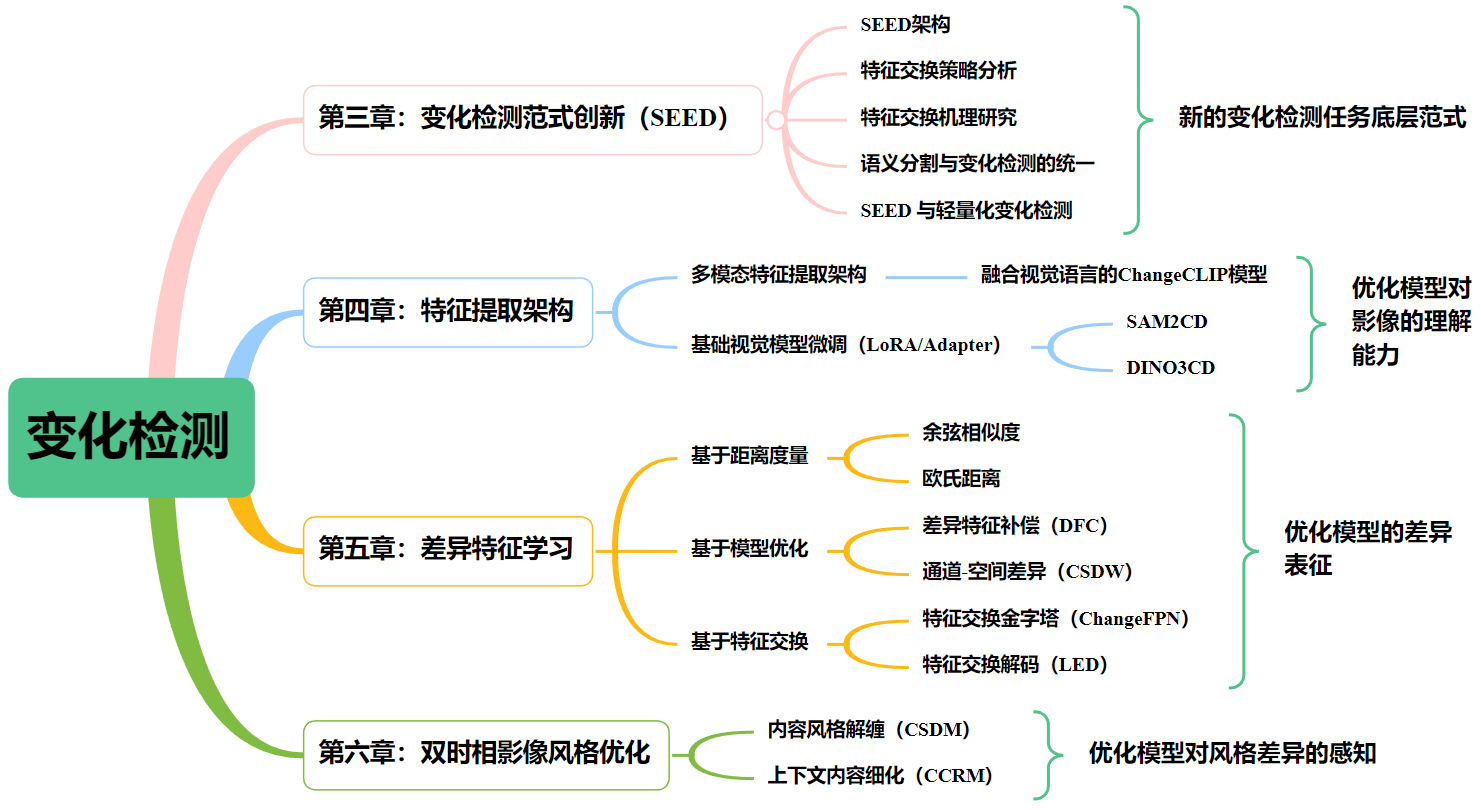
\includegraphics[width=\textwidth]{paper_figures/绪论/研究内容关联.png}
  \caption{研究内容及其关联性}
  \label{fig:research_content}
\end{figure}


\section{研究内容及其关联性}
本研究主要聚焦于基于特征交换的高分辨率遥感影像变化检测方法的创新与优化。对于常规的计算机视觉任务而言,通常有如下的研究方向,首先是加强模型的特征提取能力,构建更强大的特征提取架构,增强模型的特征拟合能力,比如VGG~\cite{Simonyan2014VeryDC}、ResNet~\cite{He2015DeepRL}以及ViT~\cite{Dosovitskiy2020AnII}等骨架模型。其次是针对具体的视觉任务,设计加强特征学习能力的模块,比如DeeplabV3plus~\cite{chen2018encoder}、PSPNet~\cite{Zhao2016PyramidSP}以及EMANet~\cite{Li2019ExpectationMaximizationAN}等模型。此外也可以根据具体的视觉任务,设计全新的模型架构,比如FCN~\cite{Shelhamer2014FullyCN}、UNet~\cite{Ronneberger2015UNetCN}以及SETR~\cite{Zheng2020RethinkingSS}等模型。根据上述常规的计算机视觉算法优化研究思路,本文在变化检测任务上围绕上述的思路进行了研究,如图~\ref{fig:research_content}所示。针对变化检测任务,本文从\textbf{变化检测架构设计优化变化检测模型对变化特征的表征方式}、\textbf{特征提取强化提升变化检测模型的对双时相影像的表征能力}、\textbf{双时相特征交互优化变化检测模型对差异特征的学习能力}以及\textbf{双时相影像风格优化减弱变化检测任务风格噪声的影响}四个方面展开了研究。

\subsection{变化检测范式创新}
现有多数变化检测架构沿用“孪生编码—差异计算—解码”的范式,其核心在于显式构造差异特征。不同于此,本文提出孪生-编码-交换-解码(\textbf{Siamese-Encoder-Exchange-Decoder,SEED})基础架构:在共享权重的孪生编码器提取出双时相多尺度特征金字塔后,\textbf{不进行任何显式差分运算},而是于进入解码阶段前执行\textbf{特征交换}(可采用特征层、空间以及通道交换),使两个孪生解码器均接收由\(T_1\)与\(T_2\)混合而成的特征序列,并使用同一变化标注进行监督。该设计将“变化”的定义由手工设定的差异特征学习,转化为模型对\textbf{双时相特征不一致性}的\textbf{隐式判别}。未变化区域在交换后的解码端保持语义—空间一致,则在模型学习中被判别为背景区域。而发生变化的区域在解码端呈现双时相影像特征的语义冲突,从而被网络自适应分割出来。SEED舍弃显式差异计算模块,结构更为简洁、参数与计算更友好,同时避免了固定运算(如相减/拼接)可能带来的信息损失,充分发挥深层网络在端到端学习\textbf{一致性/不一致性}判别上的优势。综上,此部分从理论和实验上证明了特征交换策略在变化检测任务中的有效性,为后文的模型优化奠定了基础。

\subsection{基于 AI 基础模型的变化检测特征提取强化}
针对变化检测中单一模态语义先验不足、模型泛化受限的问题,本文从\textbf{多模态视觉—语言}与\textbf{基础模型参数高效适配}两条路径强化特征提取能力。一方面,本文构建基于CLIP模型的多模态特征提取范式:利用CLIP对双时相遥感影像进行无监督语义推理,生成类别相关的文本提示,并在编码—解码框架中通过低秩双线性注意力将图像特征与文本特征进行融合,从而显式补充遥感影像的\textbf{语义信息},提升模型对复杂遥感影像的辨识能力。另一方面,面向SAM与DINO等视觉基础模型,本文提出结合视觉基础模型参数高效微调(PEFT)策略的变化检测模型PeftCD。在冻结预训练参数的前提下,通过LoRA/Adapter轻量化微调分支注入任务相关表征,有效保留大规模预训练的通用先验并使得模型充分学习到遥感影像相关知识。其中,PeftCD在变化检测范式上采用SEED架构,以此验证了SEED架构的有效性。综上,本文以\textbf{“多模态语义注入+视觉基础模型PEFT适配”}两条路径协同强化特征提取,有效缓解了单一模态语义先验不足与传统视觉模型泛化受限的问题。

\subsection{基于双时相特征交互的差异特征学习}
通常认在变化检测任务中,双时相特征交互是指利用双时相影像提取的特征,通过某种计算方法提取出能表征双时相影像差异的步骤。因此,双时相特征交互是由输入对迈向“学习变化表征”的关键步骤,。本文从互补的三个维度开展设计:(i)\textbf{差异特征计算}:围绕“如何更准确的表达双时相特征的差异”,本文在简单运算(差/和/拼接)之上,提出了基于距离度量方式(欧氏距离、余弦相似度距离)的差异特征学习模块;(ii)\textbf{结合模型设计的差异特征表达方法}: 围绕如何使用网络模块来更好的表达双时相特征的差异性,本文提出了结合空间和通道差异的差异表征方法,将变化检测任务中普遍存在的空间差异特征拓展到了空间-通道相结合的差异特征。(iii)\textbf{特征交换机制}:基于双时相影像\textbf{同地理位置}的先验,设计了基于特征层的双时相影像特征交换策略,在不显式施加差分约束的前提下,促进两时相特征的信息相互流动,使\textbf{语义不一致性}在双时相混合表征中自发显现。这三类机制分别从“显式度量差异”、“模型拟合差异”和“隐式表征差异”出发,在训练时以同一变化监督进行统一优化。

\subsection{双时相影像内容风格解缠}

针对双时相遥感影像因光照、季节等因素造成的风格差异(域偏移)干扰变化检测精度的问题,本文提出了一种基于内容-风格解耦与内容细化的变化检测网络(Content Style Disentanglement Network,CSDNet)。该模型显式分离内容特征与风格特征,并利用门控机制对风格信息进行自适应筛选,在有效抑制无关噪声的同时保留对变化判别有益的纹理等细节。具体而言,CSDNet首先通过内容-风格解缠模块(CSDM)将双时相影像特征分解为内容特征和风格特征。然后,设计了通道-空间门控机制(CSGM)对风格特征进行动态筛选,抑制无关风格信息并保留有助于变化识别的细节。最后,将筛选后的风格特征与内容特征融合,生成更鲁棒的变化表征。通过这种方式,CSDNet有效减弱了风格差异对变化检测的干扰,提高了模型在复杂场景下的精度和泛化能力。此外,本文提出的CSDNet同样采用SEED架构,再次验证了SEED架构在复变化检测任务中的有效性。



综上所述,本文的创新之处可总结如下:
\begin{enumerate}[label=(\arabic*)]
  \item  基础范式革新 (第三章): 基于特征交换策略,提出了新型的孪生-编码-交换-解码(Siamese-Encoder-Exchange-Decoder,SEED)架构,摆脱了变化检测对显式“差异计算”的依赖,通过特征交换机制驱动模型隐式学习特征不一致性,不仅简化了变化检测范式,还统一了变化检测与语义分割的框架。

  \item  特征提取强化 (第四章): 通过引入多模态信息和利用视觉基础模型进行参数高效微调,提出了首个多模态变化检测模型ChangeCLIP 以及基于视觉基础模型微调的变化检测模型 PeftCD,有效的将AI大模型与变化检测任务进行结合,提升了变化检测任务的算法效果。

  \item  双时相特征交互 (第五章): 深入研究了“差异表征”这一核心问题,从数学度量、特征交换以及多维差异等方面提出了促使模型表征差异的解决方案(EfficientCD、LENet),有效的强化了模型对变化的感知能力,提升了变化检测任务的算法效果。

  \item  伪变化抑制 (第六章): 结合SEED架构,创新性地提出了内容-风格解缠的思想(Content Style Disentanglement Network,CSDNet),通过CSDNet模型,在特征层面主动分离并过滤由光照、季节等引起的风格噪声,显著提升了模型对域差异样本的鲁棒性。
\end{enumerate}

\begin{figure}[!htbp]
  \centering
  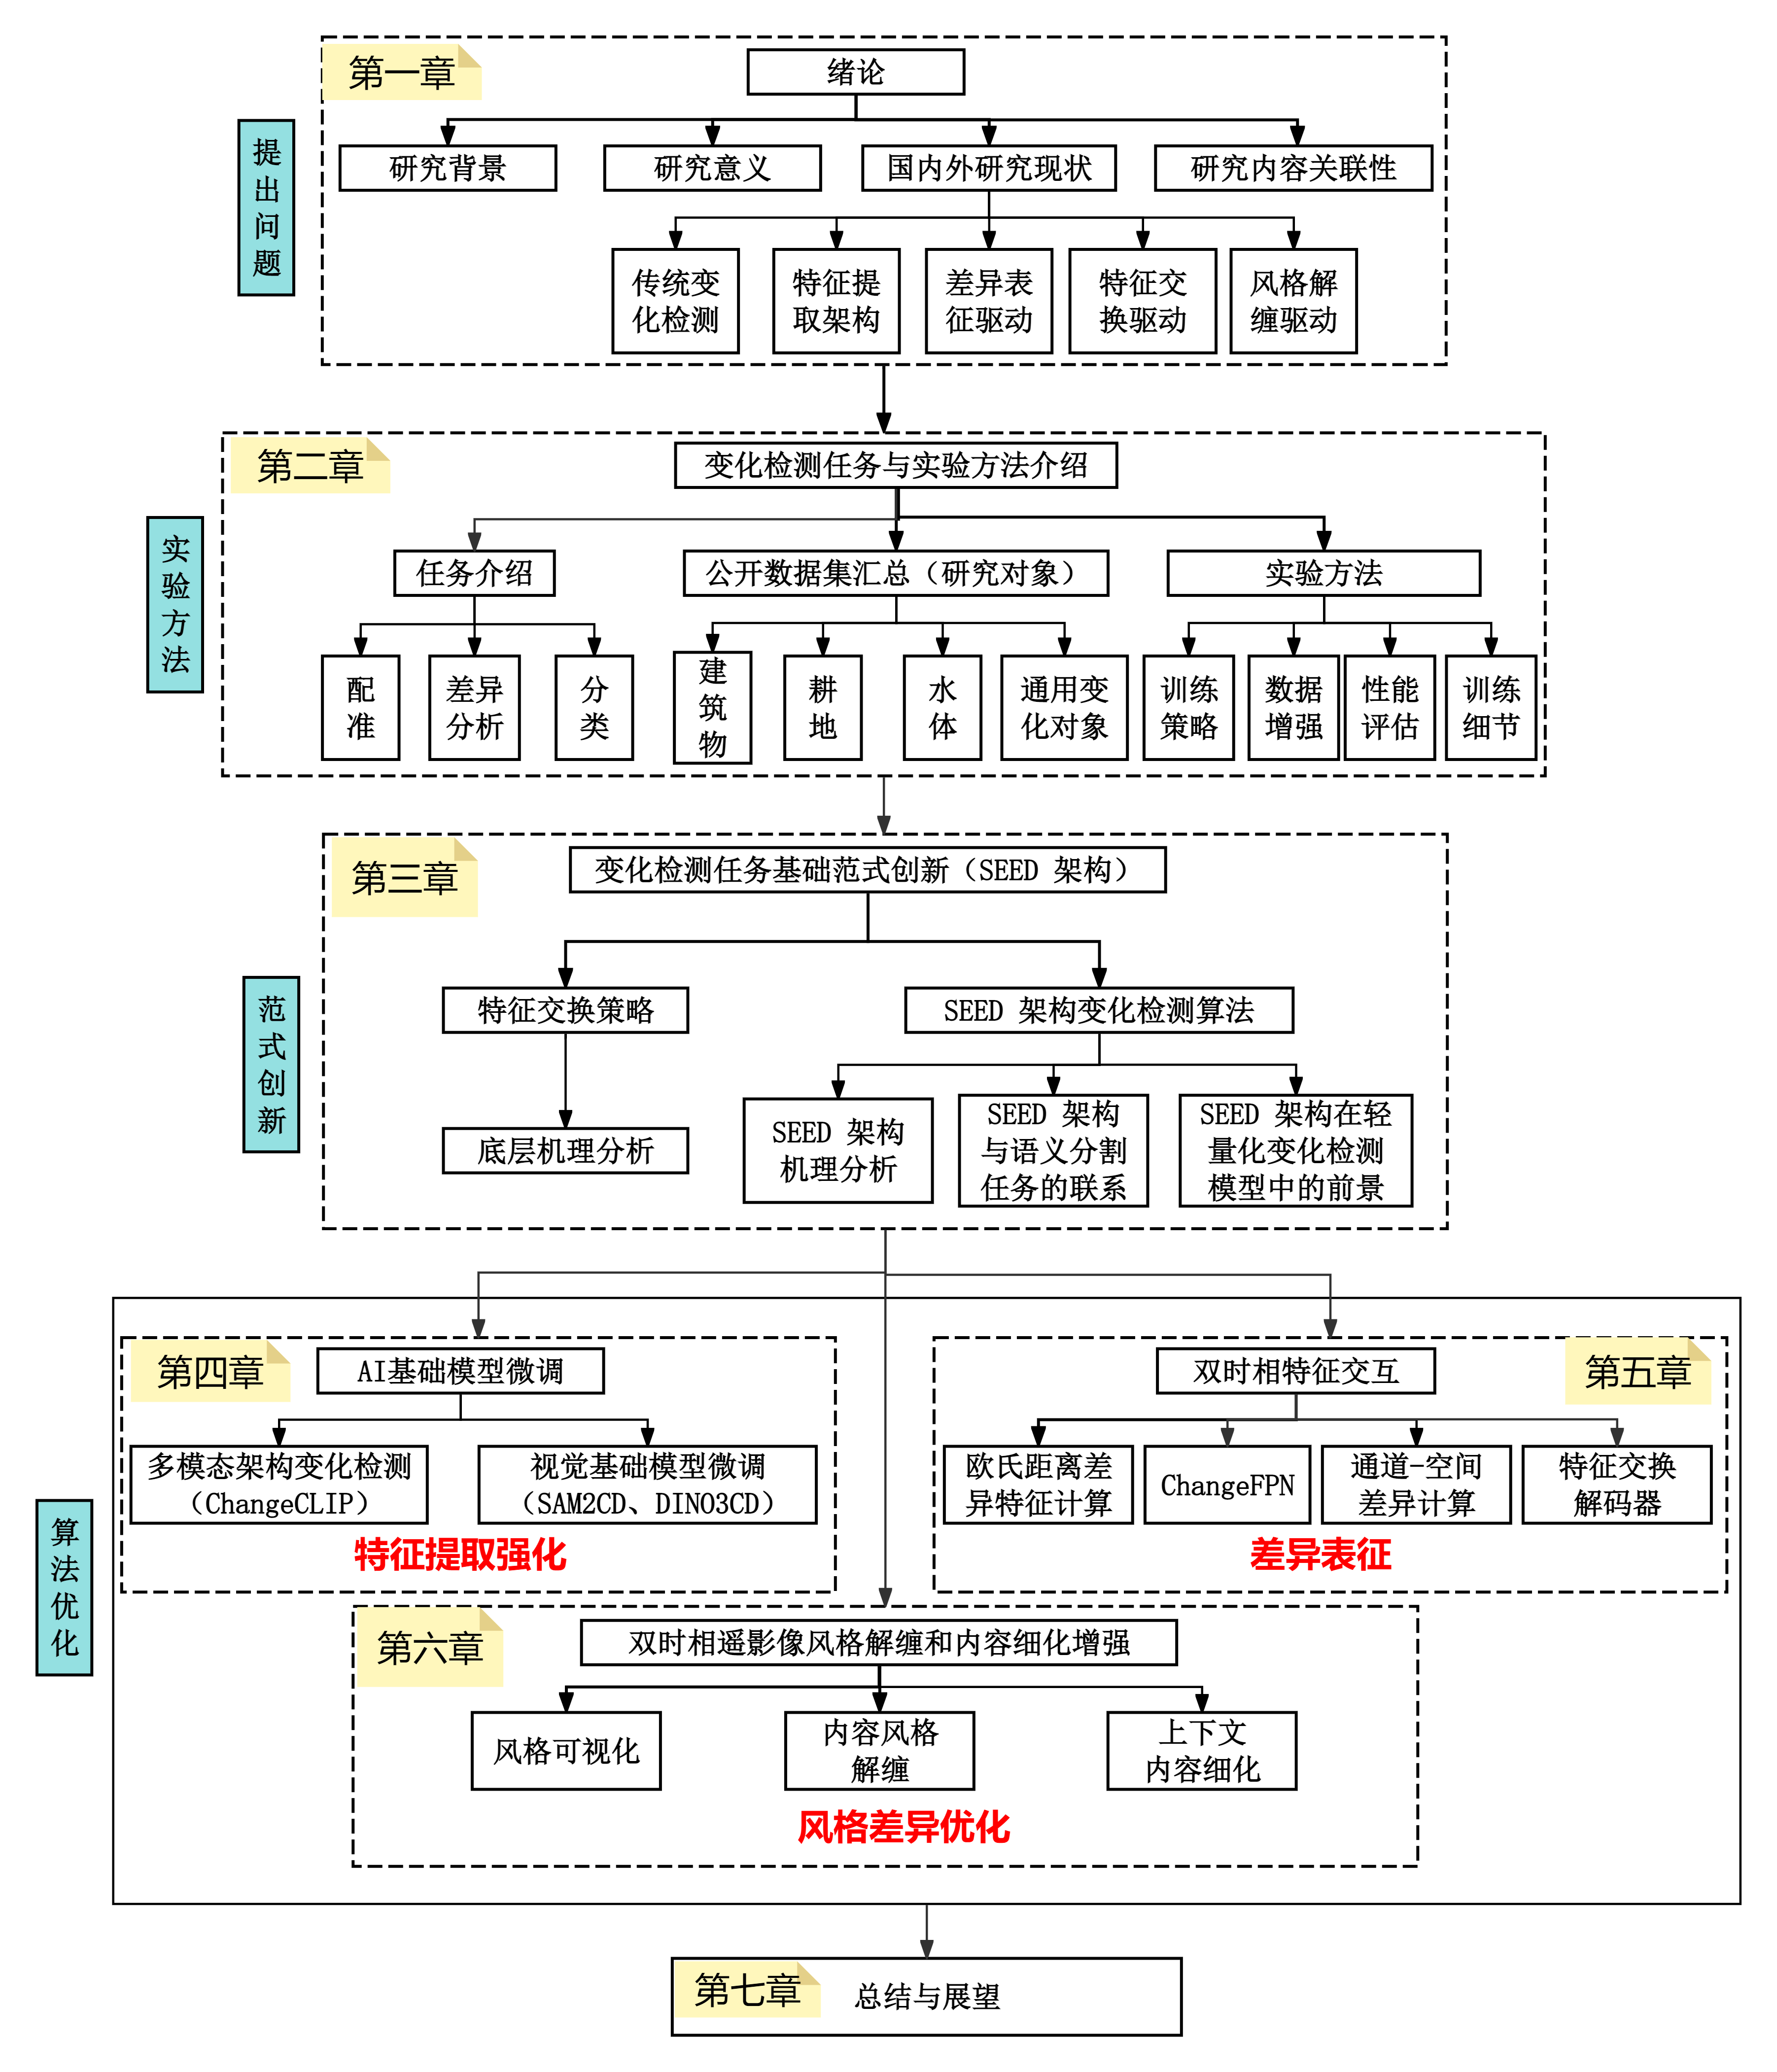
\includegraphics[width=\textwidth]{paper_figures/绪论/论文章节技术路线图.png}
  \caption{论文技术路线}
  \label{fig:paper_overall}
\end{figure}

\section{论文组织结构}
综上,本文的技术路线如图~\ref{fig:paper_overall}所示,整体分为四个层面逐步展开。首先,在绪论部分明确研究背景、意义及国内外研究现状,提出高分辨率遥感影像变化检测中存在的关键问题。其次,在实验方法部分,介绍了变化检测任务的具体实验方法。包括本文使用的多种类的数据集以及实验条件,为后文的算法设计提供了基础。随后,针对于变化检测任务范式创新,提出了Siamese-Encoder-Exchange-Decoder (SEED) 框架,以特征交换为核心机制,突破传统依赖显式差异计算的模式,实现了对变化检测任务的新型范式重构。后文的部分模型围绕SEED架构进行设计,由此证明了SEED架构的有效性。接着,本文从特征提取强化、双时相特征交互以及伪变化抑制三个方面对变化检测任务进行算法优化。在特征提取部分,论文围绕如何提升模型的特征提取能力展开,提出了基于AI基础模型微调的ChangeCLIP和PeftCD模型。在双时相特征交互部分,论文围绕如何更好的表征双时相影像的差异性展开,提出了基于距离度量的EfficientCD以及融合了通道与空间维度的(Layer-Exchange Network,LENet)。在伪变化抑制部分,论文围绕如何减弱风格噪声对变化检测任务的影响展开,提出了基于内容-风格解缠与内容细化的CSDNet模型。在此基础上,论文通过总结与展望进一步指出未来在多模态融合、跨域泛化及大规模基础模型适配等方向的研究潜力。本文的各个章节安排如下:

\textbf{第一章,绪论}。 本章首先阐述了高分辨率遥感影像变化检测的研究背景、重要意义以及当前面临的关键挑战。随后,系统回顾了变化检测算法的发展历程,涵盖了变化检测特征提取架构从传统方法到深度学习中CNN、Transformer、Mamba及AI基础模型的演进。在此基础上,进一步剖析了以差异表征和特征交换为核心的两种主流技术路线。最后,明确了本文的研究内容、核心贡献与总体技术框架,并概述了全文的组织结构。

\textbf{第二章,变化检测任务与实验方法介绍}。 本章为后续的算法研究与验证奠定基础。首先,详细介绍了本文实验所采用的多个公开变化检测数据集,涵盖了建筑物、农田、水体及通用场景等多种变化类型。接着,系统阐述了变化检测的标准实验流程,包括模型训练策略、数据增强技术以及精度验证所使用的各项性能评估指标。

\textbf{第三章,基于特征交换的变化检测基础范式创新设计}。 本章提出了一个颠覆性的变化检测基础架构——SEED (Siamese-Encoder-Exchange-Decoder)。该范式摒弃了传统的差异特征计算模块,仅通过特征交换来驱动模型学习双时相特征的不一致性。本章深入探讨了该范式背后的“像素一致性原则”,并通过实验证明了其在简化模型设计、变化检测轻量化架构、统一变化检测与语义分割任务方面的巨大潜力和卓越性能。此外,本章针对变化检测特征交换的理论和实验证明,为后续模型设计提供了坚实的理论和实验基础。

\textbf{第四章,基于AI基础模型微调的变化检测模型研究}。 本章聚焦于利用AI基础模型的强大先验知识来强化变化检测的特征提取能力。内容分为两个核心部分:第一部分介绍ChangeCLIP模型,探索了将多模态视觉-语言模型(CLIP)引入变化检测任务的方法;第二部分介绍PeftCD模型,研究了如何通过参数高效微调(PEFT)技术,将多种视觉基础模型高效适配于遥感变化检测场景,并对不同基础模型的性能进行了系统性比较。

\textbf{第五章,基于双时相遥感影像特征交互的变化检测算法研究}。 本章重点研究以“差异表征”为核心的双时相特征交互机制。内容涵盖了多种创新的差异特征计算模块,包括基于交互注意力机制的ISANet、基于距离度量的EfficientCD以及融合了通道与空间维度的LENet。通过详尽的对比实验与消融分析,验证了这些差异学习策略在提升模型对复杂变化感知能力方面的有效性。

\textbf{第六章,基于双时相遥感影像风格解缠和内容细化增强遥感变化检测方法}。 本章针对双时相遥感影像间因光照、季节等因素造成的风格差异(域偏移)干扰变化检测精度的问题,提出了一种基于内容-风格解耦与内容细化的变化检测网络(CSDNet)。该模型显式分离内容特征与风格特征,并利用门控机制对风格信息进行自适应筛选,在有效抑制无关噪声的同时保留对变化判别有益的纹理等细节。

\textbf{第七章,总结与展望}。 本章对全文的研究工作进行了全面总结,系统回顾了本文在变化检测领域的理论创新与主要贡献。在此基础上,对未来可能的研究方向进行了展望,指出了多模态融合、自监督学习、模型可解释性等领域的潜在突破口。